%%
%%
%%   askmaps.tex
%%
%%   (c)2020, J.E.J. op den Brouw <J.E.J.opdenBrouw@hhs.nl>
%%
%%   document v0.1  - 2013/12/04
%%            v0.1a - 2013/12/07
%%                  - added \karnaughmap example
%%                  - minor changes in text
%%            v0.2  - 2020/23/10
%%                  - added section on how to render covers
%%                  - changes to the text.
%%

\documentclass[a4paper,10pt]{ltxdoc}
\usepackage[a4paper,left=1.5in,right=1.5in,top=1.5in,bottom=1.5in]{geometry}

%% PDF Version and compression...
\pdfminorversion=5
\pdfobjcompresslevel=2

%% English spelling of chapter, section, etc.
\usepackage[english]{babel}

%% Use some packages
\usepackage[scaled=0.92]{helvet}
\usepackage{sansmath}
\usepackage{color}
\usepackage{float}
\usepackage{listings}
\usepackage{array}
\usepackage{tikz}
%% The next lines are commented out by default. If you want these to appear
%% in the resulting PDF, you have to have the kvmacros.tex somewhere is your
%% LaTeX search path or have a copy of the kvmacros.tex file in the
%% current directory. If so, uncomment the next lines and LaTeX this file.
%%
\input kvmacros

%% Use askmaps
\usepackage{askmaps}

%% Use hyperrefs in PDFs
\usepackage{hyperref}
\hypersetup{
  colorlinks=true,
  linkcolor=blue,
  pdftitle={American Style Karnaugh Maps},
  pdfauthor={J.E.J op den Brouw},
  pdfsubject={Drawing 1, 2, 3, 4 and 5 variables K-maps},
  pdfkeywords={K-maps, Karnaugh maps, Digital Design}
}
\definecolor{red}{rgb}{1,0,0}
\definecolor{blue}{rgb}{0,0,1}
\definecolor{darkgreen}{rgb}{0,0.4,0}
\definecolor{orange}{rgb}{1,0.5,0}
\definecolor{gray}{rgb}{0.5,0.5,0.5}
\definecolor{lightgray}{rgb}{0.95,0.95,0.95}

%% Making captions nicer...
\usepackage[font=footnotesize,format=plain,labelfont=bf,textfont=sl]{caption}
\usepackage[labelformat=simple,font=footnotesize,format=plain,labelfont=bf,textfont=sl]{subcaption}
\captionsetup[figure]{justification=centering,singlelinecheck=off,belowskip=-1ex}
\captionsetup[table]{justification=centering,singlelinecheck=off,skip=1ex}
\captionsetup[subtable]{justification=centering,singlelinecheck=off,skip=3pt}
\renewcommand\thesubfigure{(\alph{subfigure})}
\renewcommand\thesubtable{(\alph{subtable})}

%% Set up the LaTex language layout
\lstset{ %
  language=[LaTeX]tex,
  basicstyle=\footnotesize\fontfamily{pcr}\selectfont,
  commentstyle=\itshape,
  numbers=left,
  numberstyle=\tiny\color{gray},
  stepnumber=1,
  numbersep=5pt,
  %backgroundcolor=\color{lightgray},
  showspaces=false,
  showstringspaces=false,
  showtabs=false,
  frame=lines,
  rulecolor=\color{black},
  tabsize=4,
  captionpos=b,
  breaklines=true,
  breakatwhitespace=false,
  title=\lstname,
  morekeywords={RequirePackage,ProvidesPackage},
  aboveskip=\bigskipamount
}

%% Need one more footnote...
%% Display package name teletype...
\renewcommand*{\thefootnote}{\fnsymbol{footnote}}
\newcommand\Package[1]{\texttt{#1}}

%% \cmdinvoke et al politely reused from the miscdoc.sty file
\makeatletter
\DeclareRobustCommand\cmdinvoke{\@ifstar
  {\let\@tempa\emph\@scmdinvoke}%
  {\let\@tempa\relax\@scmdinvoke}%
}
\def\@scmdinvoke#1{\texttt{\symbol{92}#1}%
  \futurelet\@let@token\@cmdinvoke
}
\def\@cmdinvoke{\ifx\@let@token\bgroup
    \let\@tempb\@cmdinvoke@lbrace
  \else
    \ifx\@let@token[% ]
      \let\@tempb\@cmdinvoke@lbrack
    \else
      \ifx\@let@token(% )
        \let\@tempb\@cmdinvoke@lparen
      \else
        \let\@tempb\@empty
      \fi
    \fi
  \fi
  \@tempb
}
\def\@cmdinvoke@lbrace#1{\penalty0\hskip0pt\relax
  \texttt{\symbol{123}\@tempa{#1}\symbol{125}}%
  \futurelet\@let@token\@cmdinvoke
}
\def\@cmdinvoke@lbrack[#1]{\penalty-150\hskip0pt\relax
  \texttt{[\@tempa{#1}]}%
  \futurelet\@let@token\@cmdinvoke
}
\def\@cmdinvoke@lparen(#1){\penalty-150\hskip0pt\relax
  \texttt{(\@tempa{#1})}%
  \futurelet\@let@token\@cmdinvoke
}
\makeatother

%% No indent
\setlength{\parindent}{0pt}
\setlength{\parskip}{1ex plus 0.5ex minus 0.2ex}

%% At last, the document...
\begin{document}
\title{The \Package{askmaps} package}
\author{Jesse op den Brouw\thanks{The Hague University of Applied Sciences,
       \href{mailto:J.E.J.opdenBrouw@hhs.nl}{J.E.J.opdenBrouw@hhs.nl}}}
\date{\askmapsdate, version \askmapsversion}
\maketitle
\setcounter{footnote}{1}

\section{Abstract}
\label{sec:abstract}
This package generates configurable American style Karnaugh maps for 1, 2, 3,
4 and~5 variables as can be found in numerous books on digital design.
Note that there are many ways to draw correct Karnaugh
maps\footnote{E.g., a four-variable Karnaugh map can be drawn in 384 different
and correct ways} and this packages creates only one version.

There are more packages and examples that produce Karnaugh maps. A highly
recommendable package is written by Andreas W. Wieland\footnote{See
\url{http://www.ctan.org/tex-archive/macros/latex/contrib/karnaugh}}.
This package creates maps that are frequently found in European
textbooks\footnote{E.g. Digitale Techniek, A.P. Thijssen} but not in American
textbooks.

\section{Overview}
\label{sec:overview}
After \cmdinvoke{usepackage}[\textit{option}]{askmaps}, siz new commands are
available to draw Karnaugh maps:% using the \Package{picture} environment:
\begin{table}[H]
\begin{tabular}{p{2.8cm}p{10cm}}
\cs{askmapi}      & draws a one-variable Karnaugh map \\ 
\cs{askmapii}     & draws a two-variable Karnaugh map \\ 
\cs{askmapiii}    & draws a three-variable Karnaugh map \\ 
\cs{askmapiiialt} & draws an alternate style three-variable Karnaugh map \\ 
\cs{askmapiv}     & draws a four-variable Karnaugh map \\ 
\cs{askmapv}      & draws a five-variable Karnaugh map \\
\end{tabular} 
\end{table}

These commands have five parameters which have the same meaning for each
commands. This will be explained in Section \ref{sec:outline}. As can be seen
later on, many of the parameters can include typesetting commands such as
coloring and math notation.

The new dimension \cs{askmapunitlength} is available and specifies the length
and width of the squares. It defaults to 1 cm (about 0.4 in) which is good in
combination with a~12 pt font size.

The global definitions \cs{askmapsversion} and \cs{askmapsdate} will render
to the current version and date respectively.

There are three commands that control the size (and shape) of the rendered
text. The \cs{askmapindexsize} command sets the size and shape of the index
number, the default is \cs{scriptsize}\cs{slshape}. The \cs{askmapcontentsize} command sets
the size of the contents of the cells. It defaults to \cs{normalsize}. The
\cs{askmapbitcombinationsize} sets the the size of the bit combinations
on the edges of the Karnaugh map. It defaults to \cs{footnotesize}. These
sizes can be changed using the appropriate \cs{renewcommand} command.

The command \cs{askmapvarsep} contains the length of the variable separator
line in de Karnaugh maps. The default is 0.7. Note that it is merely a
number, not a length. It can be altered using the appropriate
\cs{renewcommand} command. See Section~\ref{sec:use} for more details.

The command \cs{askmap} provides drop-in replacement for the \cs{karnaughmap}
command available in the \Package{kvmacros} package and internally calls one
of the five commands (the \cs{askmapiiialt} command is not supported), but
there are some drawbacks on using this command.

\section{Outline}
\label{sec:outline}
%% 2013/12/07: functions -> commands
All six commands take the form
\cs{askmap<spec>\{\#1\}\{\#2\}\{\#3\}\{\#4\}\{\#5\}} where \texttt{<spec>} is
one of \texttt{i}, \texttt{ii}, \texttt{iii}, \texttt{iiialt}, \texttt{iv} or
\texttt{v} and the parameters \texttt{\#1} to \texttt{\#5} have the following
meaning:

\begin{itemize}
\itemsep0pt
\item[\texttt{\#1}] is the function output variable.
\item[\texttt{\#2}] is a list of function input variables.
\item[\texttt{\#3}] contains a list op options, see table below.
\item[\texttt{\#4}] is a list of function values.
\item[\texttt{\#5}] can be used to display user defined picture commands.
\end{itemize}

If a parameter contains fewer elements than needed, you will get empty spaces
in the Karnaugh map. If a parameter contains more elements than needed, all
elements in excess are not printed. In both situations, you will not be
notified.

The third parameter contains a list of options as explained below.
\begin{itemize}
    \itemsep0pt
    \item[\texttt{i}] index numbers are printed in the lower left corner of
                      each square.
    \item[\texttt{I}] no index numbers are printed (default).
    \item[\texttt{f}] function output variable is printed at the upper right
                      corner of the Karnaugh map together with a small line
                      extending from the square to the function
                      name (default, see Package Option Handling).
    \item[\texttt{F}] no function output variable is printed
    \item[\texttt{b}] bit combinations of the function input variables are
                      printed on top of the columns and at the left of the the
                      rows (default).
    \item[\texttt{B}] bit combinations are not printed.
    \item[\texttt{c}] shortcut for \texttt{ifb}.
    \item[\texttt{C}] shortcut for \texttt{IFB}.
\end{itemize}

Options are evaluated from left to right, so a combination of \texttt{iI} will
yield in no index numbers being printed. Please note that macros are not
expanded to a list of tokens but to one token.

%%%%If you look at American style Karnaugh maps, you will see that the function
%%%%output variable usually isn't printed with the map, but is printed below or
%%%%besides the map (if it is printed at all). This behavior can be simulated by
%%%%using the \texttt{F} option, in which case the first parameter (the function
%%%%output variable) may be left unused.

\section{Package Option Handling}
\label{sec:optionhandling}
As of version 0.2, the option \texttt{disablef} disables the default rendering
of the function output variable at the upper right corner of the Karnaugh map
together with a small line extending from the square to the function name
(option \texttt{f} in the third parameter). This is more common found in
American textbooks.


\section{Use}
\label{sec:use}
Let's say we have the following truth table for a function S with two variables
a and b and the function values 1, 0, 1 and 1 respectively.

\begin{table}[H]
\centering
\caption{A truth table.}
\begin{tabular}{cc|c}
%\hline 
a & b & S \\ \hline 
0 & 0 & 1 \\ 
0 & 1 & 0 \\ 
1 & 0 & 1 \\ 
1 & 1 & 1 \\ 
%\hline 
\end{tabular} 
\end{table}

The command
\begin{verbatim}
  \askmapii{S}{ab}{i}{1011}{}
\end{verbatim}
will produce the two-variable Karnaugh map as presented in
Figure~\ref{fig:askmapii}.
\begin{figure}[h]
\centering
\askmapunitlength=0.88cm
\askmapii{S}{ab}{i}{1011}{}%
\caption{Karnaugh map for two variables.}
\label{fig:askmapii}
\end{figure}

As you can see, the function output variable is printed top right of the
Karnaugh map, with a small line from the variable to the top right square.
The most significant function input variable is printed on the top left just
above the small line extending from the top left square (the variable
separator line). The least significant
function input variable is printed just below that line. The bit combinations
for the most significant function input variables are printed on top of the
columns, the bit combinations of the least significant function input variable
are printed left of the rows. You can see how the function values are
placed in the squares by observing the small index numbers in the lower left
corners of the squares.
\medskip

The command 
\begin{verbatim}
  \askmapiii{S}{abc}{}{10110110}{}
\end{verbatim}
will produce a three-variable Karnaugh map as presented in
Figure~\ref{fig:askmapiii}. In this case, the index numbers are not printed.

\begin{figure}[H]
\centering
\askmapunitlength=0.88cm
\askmapiii{S}{abc}{}{10110110}{}%
\caption{Karnaugh map for three variables.}
\label{fig:askmapiii}
\end{figure}

Sometimes you need a three-variable Karnaugh map that is printed in the
vertical direction. It will leave you room to print accompanying text to
the left or right of the map. The command

\begin{verbatim}
  \askmapiiialt{S}{abc}{}{10110110}{}
\end{verbatim}
will produce the vertical oriented version of the three-variable Karnaugh map
as can been seen in Figure~\ref{fig:askmapiiialt}.

\begin{figure}[H]
\centering
\askmapunitlength=0.88cm
\askmapiiialt{S}{abc}{}{10110110}{}%
\caption{Vertical version of the Karnaugh map for three variables.}
\label{fig:askmapiiialt}
\end{figure}

Let's draw a Karnaugh map for a logic function with four inputs.
The output will become logic~1 if three or four inputs are logic 1, otherwise
the output is logic 0. (Of course you can set up a truth table first; this is
left as an exercise to the reader).
The command 
\begin{verbatim}
  \askmapiv{S}{abcd}{}{0000000100010111}{}
\end{verbatim}
will produce a four-variable Karnaugh map for the given logic function and is
presented in Figure~\ref{fig:askmapiv}.

\begin{figure}[H]
\centering
\askmapunitlength=0.88cm
  \askmapiv{S}{abcd}{}{0000000100010111}{}
\caption{Karnaugh map for four variables.}
\label{fig:askmapiv}
\end{figure}

Using the command
\begin{verbatim}
  \askmapv{S}{abcde}{}{00101101010010111011110011101011}{}
\end{verbatim}
a five-variable Karnaugh map is produced as shown in Figure~\ref{fig:askmapv}.

\begin{figure}[H]
\centering
\askmapunitlength=0.88cm
  \askmapv{S}{abcde}{}{00101101010010111011110011101011}{}
\caption{Karnaugh map for five variables.}
\label{fig:askmapv}
\end{figure}

Of course you can do a lot more with the arguments of the commands. You
can use inline math to produce sophisticated variable names, you can
use coloring for the function values. However, please note that the second
and fourth parameter act as a list of tokens, so you have to use braces to
separate the tokens in the lists if they consists of multiple characters.
A list of tokens such as
\begin{verbatim}
  {abcd}
\end{verbatim}
will yield a, b, c and d as separate tokens, but
\begin{verbatim}
  {$m_{0}$$m_{1}$$m_{0}$$m_{1}$}
\end{verbatim}
will not work. You have to write
\begin{verbatim}
  {{$m_{0}$}{$m_{1}$}{$m_{0}$}{$m_{1}$}}
\end{verbatim}

The fifth parameter can be used to supply user created picture commands
such as dashed rectangles or ovals to emphasize the simplifications in the
function. Note that the origin of the picture (0,0) is at the lower left
corner of the lower left square. Sections~\ref{sec:drawing} and~%
\ref{sec:examples} show some examples.
\bigskip

%%%The size of the indexes is scriptsize, the size of the bit combinations
%%%on the edges of the Karnaugh maps is footnotesize. All other text is
%%%in normalsize. Note that there are no commands to change the font sizes
%%%in the Karnaugh maps.
%%%\bigskip


The command \cs{askmap} provides a drop-in replacement for the command
\cs{karnaughmap} from the Karnaugh package. The command
\begin{verbatim}
  \askmap{4}{S}{abcd}{0100101010100011}{}
\end{verbatim}
produces the Karnaugh map in Figure \ref{fig:askmap}.
\begin{figure}[H]
\centering
\askmapunitlength=0.88cm
  \askmap{4}{S}{abcd}{0100101010100011}{}
\caption{Karnaugh map using drop-in replacement.}
\label{fig:askmap}
\end{figure}

Note that when using this command the output function variable is always
printed.

Only Karnaugh maps of one to five variables are supported, any other number
will trigger a warning. Please note that \cs{kvindex} and \cs{kvnoindex} are
supported as can be seen in Figure~\ref{fig:karnaughmapindex}, but
\cs{kvindexsize} and \cs{kvcontentsize} commands are not supported.
\begin{verbatim}
  \kvindex
  \askmap{4}{f(a,b,c,d):}{abcd}{1110011001100110}{}
\end{verbatim}
\begin{figure}[H]
\centering
\askmapunitlength=0.88cm
  \kvindex
  \askmap{4}{f(a,b,c,d):}{abcd}{1110011001100110}{}
\caption{Karnaugh map using the \Package{kvmacros} package.}
\label{fig:karnaughmapindex}
\end{figure}

%% The next lines are commented out by default. If you want these to appear
%% in the resulting PDF, you have to copy the kvmacros.tex file in the
%% current directory, uncomment the next lines and LaTex this file.
%%
The packages \Package{kvmacros} and \Package{askmaps} can be used in the same
document as shown in Figure \ref{fig:karnaughmapnoindex}.
\begin{verbatim}
  \kvnoindex
  \karnaughmap{4}{f(a,b,c,d):}{abcd}{1110011001100110}{}
\end{verbatim}
\begin{figure}[H]
\centering
  \kvnoindex
  \karnaughmap{4}{f(a,b,c,d):}{abcd}{1110011001100110}{}
\caption{Karnaugh map using the \Package{kvmacros} package.}
\label{fig:karnaughmapnoindex}
\end{figure}

The lenght of the line separating the input variables can be set to a
different value as shown in Figure~\ref{fig:difflenvarsep}.

\begin{verbatim}
  \renewcommand{\askmapvarsep}{0.6}
  \askmapiii{S}{abc}{}{00111010}{}
  \renewcommand{\askmapvarsep}{0.9}
  \askmapiii{F}{xyz}{}{11111010}{}
\end{verbatim}
\begin{figure}[H]
\centering
\renewcommand{\askmapvarsep}{0.6}
\askmapiii{S}{abc}{}{00111010}{}
\renewcommand{\askmapvarsep}{0.9}
\askmapiii{F}{xyz}{}{11111010}{}
\caption{Different lengths of the variable separator line.}
\label{fig:difflenvarsep}
\end{figure}



\section{Drawing covers and more}
\label{sec:drawing}
One of the uses of Karnaugh maps is to simplify logic functions. The
simplifications are usually shown as (part of) circles or ovals (also squares can be used) combining
the function values that make up the simplified terms (either product terms
or sum terms).% These

Let's begin with a simple example. The code is shown below, the map is
shown in Figure~\ref{fig:kmapsthree}. Note that one function variable is
covered by all three ovals, hence it looks as if it is covered by a circle.

\begin{minipage}[c]{0.5\textwidth}
\begin{verbatim}
  \askmapiii{s}{abc}{}{00010111}{%
  \put(2.5,1.0){\oval(0.8,1.8)}%
  \put(2.0,0.5){\oval(1.8,0.8)}%
  \put(3.0,0.5){\oval(1.8,0.8)}%
  }%
\end{verbatim}
\end{minipage}\hfill%
\begin{minipage}[c]{0.5\textwidth}
\begin{figure}[H]
\centering
\askmapunitlength=0.88cm
\askmapiii{s}{abc}{}{00010111}{%
\put(2.5,1.0){\oval(0.8,1.8)}%
\put(2.0,0.5){\oval(1.8,0.8)}%
\put(3.0,0.5){\oval(1.8,0.8)}%
}%
\caption{Karnaugh map for three variables.}
\label{fig:kmapsthree}
\end{figure}
\end{minipage}
\bigskip

Function values on the edges of Karnaugh maps can be combined in one term.
The values are not adjacent in the maps so covering oval or circle has to be
split. This is shown in Figure~\ref{fig:kmapsthreemarkedges}. The code is
shown left. As can be seen, for marking the edges only half a circle has to
be drawn. Note the lines extending the edges of the map.


\bigskip
\begin{minipage}[c]{0.5\textwidth}
\begin{verbatim}
  \askmapiii{s}{abc}{}{11100111}{%
  \put(2.5,1.0){\oval(0.8,1.8)}%
  \put(1.0,1.5){\oval(1.8,0.8)}%
  \put(3.5,0.5){\oval(0.8,0.8)[l]}%
  \put(3.5,0.9){\line(1,0){0.7}}%
  \put(3.5,0.1){\line(1,0){0.7}}%
  \put(0.5,0.5){\oval(0.8,0.8)[r]}%
  \put(0.5,0.9){\line(-1,0){0.7}}%
  \put(0.5,0.1){\line(-1,0){0.7}}%
  }%
\end{verbatim}
\end{minipage}\hfill%
\begin{minipage}[c]{0.5\textwidth}
\vspace*{-3\baselineskip}
\begin{figure}[H]
\centering
\askmapiii{s}{abc}{}{11100111}{%
\put(2.5,1.0){\oval(0.8,1.8)}%
\put(1.0,1.5){\oval(1.8,0.8)}%
\put(3.5,0.5){\oval(0.8,0.8)[l]}%
\put(3.5,0.9){\line(1,0){0.7}}%
\put(3.5,0.1){\line(1,0){0.7}}%
\put(0.5,0.5){\oval(0.8,0.8)[r]}%
\put(0.5,0.9){\line(-1,0){0.7}}%
\put(0.5,0.1){\line(-1,0){0.7}}%
}%
\caption{Example of how to mark edges.}
\label{fig:kmapsthreemarkedges}
\end{figure}
\end{minipage}
\bigskip

Making ``square'' ovals doesn't always produce a good result as can be seen
in Figure~\ref{fig:kmapsquareoval}. The column second to the right seems to
be covered by it's own oval.

\bigskip
\begin{minipage}[c]{0.5\textwidth}
\begin{verbatim}
  \askmapiii{s}{abc}{}{00111111}{%
  \put(2.5,1.0){\oval(0.8,1.8)[rb]}%
  \put(2.5,1.0){\oval(0.8,1.8)[rt]}%
  \put(1.5,1.0){\oval(0.8,1.8)[lb]}%
  \put(1.5,1.0){\oval(0.8,1.8)[lt]}%
  \put(1.5,1.9){\line(1,0){1.0}}%
  \put(1.5,0.1){\line(1,0){1.0}}%
  \put(3.5,1.0){\oval(0.8,1.8)[rb]}%
  \put(3.5,1.0){\oval(0.8,1.8)[rt]}%
  \put(2.5,1.0){\oval(0.8,1.8)[lb]}%
  \put(2.5,1.0){\oval(0.8,1.8)[lt]}%
  \put(2.5,1.9){\line(1,0){1.0}}%
  \put(2.5,0.1){\line(1,0){1.0}}%
  }%
\end{verbatim}
\end{minipage}\hfill%
\begin{minipage}[c]{0.5\textwidth}
\vspace*{-3\baselineskip}
\begin{figure}[H]
\centering
\askmapiii{s}{abc}{}{00111111}{%
\put(2.5,1.0){\oval(0.8,1.8)[rb]}% the square oval
\put(2.5,1.0){\oval(0.8,1.8)[rt]}% in the middle
\put(1.5,1.0){\oval(0.8,1.8)[lb]}% of the map
\put(1.5,1.0){\oval(0.8,1.8)[lt]}%
\put(1.5,1.9){\line(1,0){1.0}}%
\put(1.5,0.1){\line(1,0){1.0}}%
\put(3.5,1.0){\oval(0.8,1.8)[rb]}% the square oval
\put(3.5,1.0){\oval(0.8,1.8)[rt]}% on the right
\put(2.5,1.0){\oval(0.8,1.8)[lb]}% of the map
\put(2.5,1.0){\oval(0.8,1.8)[lt]}%
\put(2.5,1.9){\line(1,0){1.0}}%
\put(2.5,0.1){\line(1,0){1.0}}%
}%
\caption{Example of bad use of ovals.}
\label{fig:kmapsquareoval}
\end{figure}
\end{minipage}
\bigskip





Let's try a four-variable map, see Figure~\ref{fig:kmapsthreemarkedges2}
and accompanying code. Here we have deliberately used an oval with a
bigger size (see code line marked \textasteriskcentered) otherwise it will
interfere with the covering of the lower left and right edges. An example
of good use of a ``square'' oval can be found in
Figure~\ref{fig:kmapforfourvarcorner}.

\bigskip
\begin{minipage}[c]{0.5\textwidth}
\begin{verbatim}
  \askmapiv{s}{abcd}{}{0111010001110111}{%
  \put(2.0,2.5){\oval(3.8,0.8)}%
  \put(0.5,1.0){\oval(0.8,1.8)[rb]}%
  \put(0.5,1.0){\oval(0.8,1.8)[rt]}%
  \put(0.5,1.9){\line(-1,0){0.7}}%
  \put(0.5,0.1){\line(-1,0){0.7}}%
  \put(3.0,1.0){\oval(1.8,1.8)}% (*)
  \put(3.5,1.0){\oval(0.8,1.8)[lb]}%
  \put(3.5,1.0){\oval(0.8,1.8)[lt]}%
  \put(3.5,1.9){\line(1,0){0.7}}%
  \put(3.5,0.1){\line(1,0){0.7}}%
  }%
\end{verbatim}
\end{minipage}\hfill%
\begin{minipage}[c]{0.5\textwidth}
\vspace*{-2\baselineskip}
\begin{figure}[H]
\centering
\askmapiv{s}{abcd}{}{0111010001110111}{%
\put(2.0,2.5){\oval(3.8,0.8)}%
\put(0.5,1.0){\oval(0.8,1.8)[rb]}%
\put(0.5,1.0){\oval(0.8,1.8)[rt]}%
\put(0.5,1.9){\line(-1,0){0.7}}%
\put(0.5,0.1){\line(-1,0){0.7}}%
\put(3.0,1.0){\oval(1.8,1.8)}%
\put(3.5,1.0){\oval(0.8,1.8)[lb]}%
\put(3.5,1.0){\oval(0.8,1.8)[lt]}%
\put(3.5,1.9){\line(1,0){0.7}}%
\put(3.5,0.1){\line(1,0){0.7}}%
}%
\caption{Example of how to mark edges.}
\label{fig:kmapsthreemarkedges2}
\end{figure}
\end{minipage}
\bigskip



Every textbook on using Karnaugh maps shows how to combine the corners of a
four-variable map. The complete code is shown below. The result is shown in
Figure~\ref{fig:kmapforfourvarcorner}. Each corner marking
consists of three drawing command: two lines (to the left, right up or
down) and one (part of a) oval (right-bottom, left-bottom, right-top
and right-bottom).


\begin{verbatim}
  \begin{figure}[H]
  \centering
  \askmapiv{s}{abcd}{}{1010000010100000}{%
  \put(0.5,3.5){\oval(0.8,0.8)[rb]}% left-top
  \put(0.5,3.1){\line(-1,0){0.7}}%
  \put(0.9,3.5){\line(0,1){0.7}}%
  \put(3.5,3.5){\oval(0.8,0.8)[lb]}% right-top
  \put(3.5,3.1){\line(1,0){0.7}}%
  \put(3.1,3.5){\line(0,1){0.7}}%
  \put(0.5,0.5){\oval(0.8,0.8)[rt]}% left-bottom
  \put(0.5,0.9){\line(-1,0){0.7}}%
  \put(0.9,0.5){\line(0,-1){0.7}}%
  \put(3.5,0.5){\oval(0.8,0.8)[lt]}% right-bottom
  \put(3.5,0.9){\line(1,0){0.7}}%
  \put(3.1,0.5){\line(0,-1){0.7}}%
  \put(2.5,2.0){\oval(0.8,1.8)[rb]}% the square oval
  \put(2.5,2.0){\oval(0.8,1.8)[rt]}% in the middle
  \put(1.5,2.0){\oval(0.8,1.8)[lb]}% of the map
  \put(1.5,2.0){\oval(0.8,1.8)[lt]}%
  \put(1.5,2.9){\line(1,0){1.0}}%
  \put(1.5,1.1){\line(1,0){1.0}}%
  }%
  \caption{The corners of the Karnaugh map are connected.}
  \label{fig:kmapforfourvarcorner}
  \end{figure}
\end{verbatim}

\begin{figure}[H]
\centering
\askmapiv{s}{abcd}{}{1010010110100101}{%
\put(0.5,3.5){\oval(0.8,0.8)[rb]}% left-top
\put(0.5,3.1){\line(-1,0){0.7}}%
\put(0.9,3.5){\line(0,1){0.7}}%
\put(3.5,3.5){\oval(0.8,0.8)[lb]}% right-top
\put(3.5,3.1){\line(1,0){0.7}}%
\put(3.1,3.5){\line(0,1){0.7}}%
\put(0.5,0.5){\oval(0.8,0.8)[rt]}% left-bottom
\put(0.5,0.9){\line(-1,0){0.7}}%
\put(0.9,0.5){\line(0,-1){0.7}}%
\put(3.5,0.5){\oval(0.8,0.8)[lt]}% right-bottom
\put(3.5,0.9){\line(1,0){0.7}}%
\put(3.1,0.5){\line(0,-1){0.7}}%
\put(2.5,2.0){\oval(0.8,1.8)[rb]}% the square oval
\put(2.5,2.0){\oval(0.8,1.8)[rt]}% in the middle
\put(1.5,2.0){\oval(0.8,1.8)[lb]}% of the map
\put(1.5,2.0){\oval(0.8,1.8)[lt]}%
\put(1.5,2.9){\line(1,0){1.0}}%
\put(1.5,1.1){\line(1,0){1.0}}%
}%
\caption{The corners of the Karnaugh map are connected.}
\label{fig:kmapforfourvarcorner}
\end{figure}


When writing a textbook on the use of Karnaugh maps, it sometimes helps if
a cover is accompanied with the term it covers.
Below is a fine example of explaining the simplification of a logic function
by showing the product term at each cover. The truth table is shown at the
right.

\begin{verbatim}
\begin{figure}[H]
\begin{subfigure}[c]{0.5\textwidth}
\centering
\askmapiii{s}{abc}{}{00010111}{%
\put(2.5,1.0){\oval(0.8,1.8)}%
\put(3.0,3.0){\makebox(0,0){$a\cdot b$}}%
\put(3.0,2.8){\line(-1,-5.0){0.2}}%
\put(2.0,0.5){\oval(1.8,0.8)}%
\put(0.5,-0.8){\makebox(0,0){$b\cdot c$}}%
\put(0.5,-0.6){\line(1,0.9){0.8}}%
\put(3.0,0.5){\oval(1.8,0.8)}%
\put(4.5,-0.8){\makebox(0,0){$a\cdot c$}}%
\put(4.5,-0.6){\line(-1,0.9){0.8}}%
}%
\end{subfigure}%
\begin{subfigure}[c]{0.5\textwidth}
\centering
\begin{tabular}{ccc|c}
$a$ & $b$ & $c$ & $s$ \\ \hline
 0  &  0  &  0  &  0  \\
 0  &  0  &  1  &  0  \\
 0  &  1  &  0  &  0  \\
 0  &  1  &  1  &  1  \\
 1  &  0  &  0  &  0  \\
 1  &  0  &  1  &  1  \\
 1  &  1  &  0  &  1  \\
 1  &  1  &  1  &  1  \\
\end{tabular}
\end{subfigure}%
\bigskip\caption{Karnaugh map for three variables.}
\label{fig:karnaughmajorfunctie}
\end{figure}
\end{verbatim}


\begin{figure}[H]
\begin{subfigure}[c]{0.5\textwidth}
\centering
\askmapunitlength=0.88cm
\askmapiii{s}{abc}{}{00010111}{%
\put(2.5,1.0){\oval(0.8,1.8)}%
\put(3.0,3.0){\makebox(0,0){$a\cdot b$}}%
\put(3.0,2.8){\line(-1,-5.0){0.2}}%
\put(2.0,0.5){\oval(1.8,0.8)}%
\put(0.5,-0.8){\makebox(0,0){$b\cdot c$}}%
\put(0.5,-0.6){\line(1,0.9){0.8}}%
\put(3.0,0.5){\oval(1.8,0.8)}%
\put(4.5,-0.8){\makebox(0,0){$a\cdot c$}}%
\put(4.5,-0.6){\line(-1,0.9){0.8}}%
}%
\end{subfigure}%
\begin{subfigure}[c]{0.5\textwidth}
\centering
\begin{tabular}{ccc|c}
$a$ & $b$ & $c$ & $s$ \\ \hline
 0  &  0  &  0  &  0  \\
 0  &  0  &  1  &  0  \\
 0  &  1  &  0  &  0  \\
 0  &  1  &  1  &  1  \\
 1  &  0  &  0  &  0  \\
 1  &  0  &  1  &  1  \\
 1  &  1  &  0  &  1  \\
 1  &  1  &  1  &  1  \\
\end{tabular}
\end{subfigure}%
\bigskip\caption{Karnaugh map for three variables.}
\label{fig:karnaughmajorfunction}
\end{figure}

A very notable feature is when you use Ti\textsl{k}Z. When you use the package with

\begin{verbatim}
\usepackage{tikz}
\end{verbatim}

you can use Ti\textsl{k}Z' opacity control to add opaque solid rectangles in the back:

\begin{verbatim}
\askmapii{F}{xy}{f}{0111}{
\setlength\fboxsep{0pt}\linethickness{0pt}
\put(1.1,0.1){\pgfsetfillopacity{0.2}\colorbox{red}{\framebox(0.8,1.8){}}\pgfsetfillopacity{1}}%
\put(0.1,0.1){\pgfsetfillopacity{0.2}\colorbox{blue}{\framebox(1.8,0.8){}}\pgfsetfillopacity{1}}%
}
\end{verbatim}

\askmapii{F}{xy}{f}{0111}{
\setlength\fboxsep{0pt}\linethickness{0pt}
\put(1.1,0.1){\pgfsetfillopacity{0.2}\colorbox{red}{\framebox(0.8,1.8){}}\pgfsetfillopacity{1}}%
\put(0.1,0.1){\pgfsetfillopacity{0.2}\colorbox{blue}{\framebox(1.8,0.8){}}\pgfsetfillopacity{1}}%
}

\bigskip
In fact, you can use a \texttt{tikzpicture} environment to use Ti\textsl{k}Z commands
but you have to set an invisible point to coordinate to (0,0):

\begin{verbatim}
\askmapii{F}{xy}{f}{0111}{%
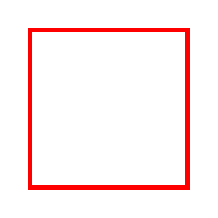
\begin{tikzpicture}[x=\askmapunitlength,y=\askmapunitlength]%
\draw[draw=none,fill=none] (0,0) -- (0,0); % Set default corner
\draw[red, ultra thick] (0,0) rectangle (2,2);%
\end{tikzpicture}%
}
\end{verbatim}

\askmapii{F}{xy}{f}{0111}{%
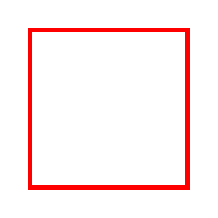
\begin{tikzpicture}[x=\askmapunitlength,y=\askmapunitlength]%
\draw[draw=none,fill=none] (0,0) -- (0,0); % Set default corner
\draw[red,ultra thick] (0,0) rectangle (2,2);%
\end{tikzpicture}%
}


\section{Additional command}
The command \cmdinvoke{askmapindexsize} sets the size and typeface of the minterm numbers in the cells. The default definition is set to

\begin{lstlisting}
\newcommand{\askmapindexsize}{\scriptsize\slshape}
\end{lstlisting}

The command \cmdinvoke{askmapcontentsize} sets the size and typeface for the cell's contents. The default definition is

\begin{lstlisting}
\newcommand{\askmapcontentsize}{\normalsize}
\end{lstlisting}

The command \cmdinvoke{askmapbitcombinationsize} sets the size and typeface for the bit combinations at the top and the left. The default definition is

\begin{lstlisting}
\newcommand{\askmapbitcombinationsize}{\footnotesize}
\end{lstlisting}

The command \cmdinvoke{askmapvarsep} sets the relative line length of the variable separator on the left of the Karnaugh map. The default definition is

\begin{lstlisting}
\newcommand{\askmapvarsep}{0.70}
\end{lstlisting}

These commands may be changed using the appropriate \cmdinvoke{renewcommand} command.


%\newpage
\section{Examples}
\label{sec:examples}
\askmapunitlength=0.88cm
The most simple Karnaugh maps you can make with only one variable.
\begin{verbatim}
  \askmapi{s}{a}{i}{00}{}
  \askmapi{s}{a}{}{01}{}
  \askmapi{s}{a}{}{10}{}
  \askmapi{s}{a}{}{11}{}
\end{verbatim}
\askmapi{s}{a}{i}{00}{}%
\askmapi{s}{a}{}{01}{}%
\askmapi{s}{a}{}{10}{}%
\askmapi{s}{a}{}{11}{}%
\bigskip\bigskip

The Karnaugh maps for two variables: plain, with indexes and output
variable.
\begin{verbatim}
  \askmapii{S}{ab}{F}{1010}{}
  \askmapii{S}{ab}{i}{1110}{}
  \askmapii{S}{ab}{}{1110}{}
\end{verbatim}
\askmapii{S}{ab}{F}{1010}{}
\askmapii{S}{ab}{i}{1110}{}
\askmapii{S}{ab}{}{1110}{}
\bigskip\bigskip

The Karnaugh maps for three variables: plain, with indexes and function
output variable.
\begin{verbatim}
  \askmapiii{S}{abc}{F}{00111010}{}
  \askmapiii{F}{xyz}{i}{11111010}{}
\end{verbatim}
\askmapiii{S}{abc}{F}{00111010}{}
\askmapiii{F}{xyz}{i}{11111010}{}
\bigskip\bigskip

The Karnaugh maps for four variables: plain, with function output variable and
indexes.
\begin{verbatim}
  \askmapiv{f}{wxyz}{F}{1110001101000101}{}
  \askmapiv{S}{abcd}{i}{1100100100011101}{}
\end{verbatim}
\askmapiv{f}{wxyz}{F}{1110001101000101}{}
\askmapiv{S}{abcd}{i}{1100100100011101}{}
\bigskip\bigskip

You can also do math things by using the known \$ signs... and you can make an
empty map for your exams...
\begin{verbatim}
  \askmapii{$S_{0}$}{{$a_{1}$}{$a_{0}$}}{}{1010}{}
  \askmapii{}{}{F}{}{}
\end{verbatim}
\askmapii{$S_{0}$}{{$a_{1}$}{$a_{0}$}}{}{1010}{}
\askmapii{}{}{F}{}{}
\bigskip\bigskip

You can do the math thing in roman upright font... and of course you can make
a \textsl{really} empty map for your exams...
\begin{verbatim}
  \askmapiii{$\mathrm{M^{n+1}_{0}}$}{{$\mathrm{M^{n}_{2}}$}{$\mathrm{M^{n}_{1}}$}
            {$\mathrm{M^{n}_{0}}$}}{}{11100111}{}
  \askmapiii{}{}{BF}{}{}
\end{verbatim}
\askmapiii{$\mathrm{M^{n+1}_{0}}$}{{$\mathrm{M^{n}_{2}}$}{$\mathrm{M^{n}_{1}}$}
          {$\mathrm{M^{n}_{0}}$}}{}{11100111}{}
\askmapiii{}{}{BF}{}{}
\bigskip\bigskip

The vertical version of the three variable map, used in a \verb|minipage|
environment:
\begin{verbatim}
\begin{minipage}[c]{0.25\textwidth}
\askmapiiialt{s}{{c$_{in}$}ab}{}{01101001}{}
\end{minipage}
\begin{minipage}[c]{0.25\textwidth}
\askmapiiialt{c$_{out}$}{{c$_{in}$}ab}{}{00010111}{}
\end{minipage}\hfill%
\begin{minipage}[c]{0.40\textwidth}
As you can see on the left, the function of the sum of the full adder cannot
be simplified as all 1's are placed diagonal in the map. This means that the
function for the sum can be expressed with XOR ports.

The carry-out function on the otherhand can be simplified.
\end{minipage}
\end{verbatim}

\begin{minipage}[c]{0.25\textwidth}
\askmapiiialt{s}{{c$_{in}$}ab}{}{01101001}{}
\end{minipage}
\begin{minipage}[c]{0.25\textwidth}
\askmapiiialt{c$_{out}$}{{c$_{in}$}ab}{}{00010111}{}
\end{minipage}\hfill%
\begin{minipage}[c]{0.40\textwidth}
As you can see on the left, the function of the sum of the full adder cannot
be simplified as all 1's are placed diagonal in the map. This means that the
function for the sum can be expressed with XOR ports.

The carry-out function on the otherhand can be simplified.
\end{minipage}

\bigskip\bigskip


You can do things with don't cares...
\begin{verbatim}
  \askmapii{S}{ab}{}{011-}{}
  \askmapiii{S}{abc}{}{001--10-}{}
\end{verbatim}
\askmapii{S}{ab}{}{011-}{}
\askmapiii{S}{abc}{}{001--10-}{}
\bigskip\bigskip

You can use colors and empty function values and variables as values too...
\begin{verbatim}
  \askmapiii{S}{abc}{}{{\color{blue}{0}}{\color{blue}{0}}{\color{red}{1}}{ }{ }
               {\color{red}{1}}{\color{blue}{0}}{ }}{}
  \askmapii{S}{ab}{}{{$i_{0}$}{$i_{1}$}{$i_{2}$}{$i_{3}$}}{}
\end{verbatim}
\askmapiii{S}{abc}{}{{\color{blue}{0}}{\color{blue}{0}}{\color{red}{1}}{ }{ }
          {\color{red}{1}}{\color{blue}{0}}{ }}{}
\askmapii{S}{ab}{}{{$i_{0}$}{$i_{1}$}{$i_{2}$}{$i_{3}$}}{}
\bigskip


You can set the font to something else ... and use sans math font ...
\begin{verbatim}
  {\fontfamily{phv}\selectfont%
  \askmapiv{S}{abcd}{}{0110111011110011}{}%
  }
  {\fontfamily{phv}\selectfont\sansmath
  \askmapiv{$Q^{n+1}_{0}$}{{$p^{n}_{1}$}{$p^{n}_{0}$}{$q^{n}_{1}$}{$q^{n}_{0}$}}
           {}{0110111011110011}{}%
  }
\end{verbatim}
{\fontfamily{phv}\selectfont%
\askmapiv{S}{abcd}{}{0110111011110011}{}%
}
{\fontfamily{phv}\selectfont\sansmath
\askmapiv{$Q^{n+1}_{0}$}{{$p^{n}_{1}$}{$p^{n}_{0}$}{$q^{n}_{1}$}{$q^{n}_{0}$}}
         {}{0110111011110011}{}%
}
\bigskip\bigskip

You can use the last parameter to create to your own picture commands. Note
that the origin of the picture (0,0) is at the lower left corner of the lower
left square. It is also possible to use \cs{raisebox} in conjuction with
horizontal spacing to adjust the placing of the left (least significant)
variable(s).

%\newpage
\begin{verbatim}
  {\fontfamily{phv}\selectfont\sansmath
  \askmapiii{F}{xy{\raisebox{2ex}{\ \ z}}}{f}{11100111}{% raise Z input
  \color{red}\put(0.1,0.1){\dashbox{0.1}(0.8,1.8){}}%
  \color{blue}\put(1.1,1.1){\dashbox{0.1}(1.8,0.8){}}%
  \color{darkgreen}\put(2.1,0.1){\dashbox{0.1}(1.8,0.8){}}%
  \color{orange}\put(0.15,1.15){\dashbox{0.1}(1.7,0.7){}}%
  }}%
  {\fontfamily{phv}\selectfont\sansmath
  \askmapiii{F}{xyz}{}{11100111}{%
  \put(0.5,1.0){\oval(0.8,1.8)}%
  \put(2.0,1.5){\oval(1.8,0.8)}%
  \put(2.5,0.5){\oval(0.8,0.8)}% circle
  \put(3.5,0.5){\oval(0.8,0.8)[l]}% these three create
  \put(3.5,0.9){\line(1,0){0.6}}% a oval open to the left
  \put(3.5,0.1){\line(1,0){0.6}}%
  }}%
\end{verbatim}
{\fontfamily{phv}\selectfont\sansmath
\askmapiii{F}{xy{\raisebox{1.5ex}{\ \ z}}}{f}{11100111}{% raise Z input
\color{red}\put(0.1,0.1){\dashbox{0.1}(0.8,1.8){}}%
\color{blue}\put(1.1,1.1){\dashbox{0.1}(1.8,0.8){}}%
\color{darkgreen}\put(2.1,0.1){\dashbox{0.1}(1.8,0.8){}}%
\color{orange}\put(0.15,1.15){\dashbox{0.1}(1.7,0.7){}}%
}}%
{\fontfamily{phv}\selectfont\sansmath
\askmapiii{F}{xyz}{}{11100111}{%
\put(0.5,1.0){\oval(0.8,1.8)}%
\put(2.0,1.5){\oval(1.8,0.8)}%
\put(2.5,0.5){\oval(0.8,0.8)}%    circle
\put(3.5,0.5){\oval(0.8,0.8)[l]}% these three create
\put(3.5,0.9){\line(1,0){0.7}}%   an oval open to the left
\put(3.5,0.1){\line(1,0){0.7}}%
}}%
\bigskip\bigskip

You can set the length of the squares, but please note that this will also
affect the rendering of the text...
\begin{verbatim}
  \askmapunitlength=1cm
  \askmapii{S}{ab}{}{1011}{}
  \askmapunitlength=0.88cm
  \askmapii{S}{ab}{}{1011}{}
  \askmapunitlength=0.8cm
  \askmapii{S}{ab}{}{1011}{}
  \askmapunitlength=0.5cm
  \askmapii{S}{ab}{}{1011}{}
\end{verbatim}

{\askmapunitlength=1cm%
\askmapii{S}{ab}{}{1011}{}%
\askmapunitlength=0.88cm%
\askmapii{S}{ab}{}{1011}{}%
\askmapunitlength=0.8cm%
\askmapii{S}{ab}{}{1011}{}%
\askmapunitlength=0.5cm%
\askmapii{S}{ab}{}{1011}{}}
\bigskip\bigskip

%\newpage
An example directly from the Karnaugh package:

\begin{verbatim}
  \kvnoindex
  \askmap{4}{$f(a,b,c,d):$}{{$a$}{$b$}{$c$}{$d$}}%
  {0110011001100110}%
  {%
  \put(0,2){\oval(1.9,1.9)[r]}
  \put(4,2){\oval(1.9,1.9)[l]}
  \put(2,0){\oval(1.9,1.9)[t]}
  \put(2,4){\oval(1.9,1.9)[b]}
  }
\end{verbatim}
{\askmapunitlength=0.88cm
\kvnoindex
\askmap{4}{$f(a,b,c,d):$}{{$a$}{$b$}{$c$}{$d$}}%
{0110011001100110}%
{%
\put(0,2){\oval(1.8,1.8)[r]}
\put(4,2){\oval(1.8,1.8)[l]}
\put(2,0){\oval(1.8,1.8)[t]}
\put(2,4){\oval(1.8,1.8)[b]}
}}

\bigskip
but please note that the ovals do not cover the logic 1's in the Karnaugh map
because the function values are placed in a different order.

One can use Ti\textsl{k}Z. Please note you have to set a default corner to
(0,0), because Ti\textsl{k}Z will create a bounding box around the the
\texttt{tikzpicture}:

\begin{verbatim}
A static hazard can be found by inspecting the Karnaugh map and see if a change
of minterms will cross implicants:

\askmapiii{F}{xyz}{}{011100100}{%
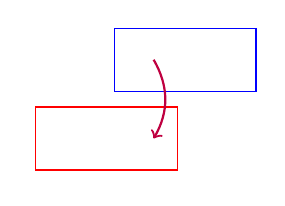
\begin{tikzpicture}[x=\askmapunitlength,y=\askmapunitlength]%
\draw[draw=none,fill=none] (0,0) -- (0,0); % Set default corner
\draw[red] (0.1,0.1) rectangle (1.9,0.9);
\draw[blue] (1.1,1.1) rectangle (2.9,1.9);
\draw[purple,thick,->] (1.6,1.5) to[bend left] (1.6,0.5);
\end{tikzpicture}%
}

The function is $F = \overline{x}z + y\overline{z}$. But if the circuit is
changing from minterm $m_2$ to $m_3$, a static hazard will occur as can
be seen by the arrow.
\end{verbatim}


A static hazard can be found by inspecting the Karnaugh map and see if a change
of minterms will cross implicants:

\askmapiii{F}{xyz}{}{011100100}{%
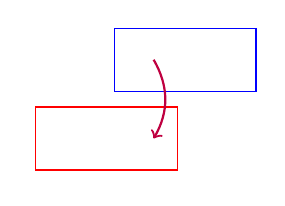
\begin{tikzpicture}[x=\askmapunitlength,y=\askmapunitlength]%
\draw[draw=none,fill=none] (0,0) -- (0,0); % Set default corner
\draw[red] (0.1,0.1) rectangle (1.9,0.9);
\draw[blue] (1.1,1.1) rectangle (2.9,1.9);
\draw[purple,thick,->] (1.6,1.5) to[bend left] (1.6,0.5);
\end{tikzpicture}%
}

The function is $F = \overline{x}z + y\overline{z}$. But if the circuit is
changing from minterm $m_2$ to $m_3$, a static hazard will occur as can
be seen by the arrow.



\section{Changelog}
\label{sec:changelog}
\begin{verbatim}
  4-dec-2013 -- v0.1
    initial release
 23-oct-2020 -- v0.2
    added option disablef
    added askmapi - a K-map for one variable
    added askmapiiialt - alternate (vertical) version op K-map III
    added formatting index size, contents size and bit combination size.
    added support for \kvindex and \nokvindex macros when kvmacros.tex is loaded
    added formatting for left-placed variables
    implemented a debug possibility
    implemented linelength of variable separator
    resolved an issue with multiple overfull \hbox'es
    added a section on creating covers
    added examples with Tikz
\end{verbatim}


\newpage
\section{The source code}
\label{sec:sourcecode}
The source code is pretty straight forward. It uses a lot of picture primitives
for drawing the maps. The package uses three macros for processing
variable-length parameters, which were completely reused from the
\Package{kvmacros} package.

\lstinputlisting{askmaps.sty}

\end{document}
